\documentclass{article}

\usepackage{amsmath,amssymb}
\usepackage{tikz}
\usepackage{pgfplots}
\usepackage{xcolor}
\usepackage[left=2.1cm,right=3.1cm,bottom=3cm,footskip=0.75cm,headsep=0.5cm]{geometry}
\usepackage{enumerate}
\usepackage{enumitem}
\usepackage{marvosym}
\usepackage{tabularx}
\usepackage{parskip}

\usepackage{listings}
\definecolor{lightlightgray}{rgb}{0.95,0.95,0.95}
\definecolor{lila}{rgb}{0.8,0,0.8}
\definecolor{mygray}{rgb}{0.5,0.5,0.5}
\definecolor{mygreen}{rgb}{0,0.8,0.26}
%\lstdefinestyle{java} {language=java}
\lstset{language=R,
	basicstyle=\ttfamily,
	keywordstyle=\color{lila},
	commentstyle=\color{lightgray},
	stringstyle=\color{mygreen}\ttfamily,
	backgroundcolor=\color{white},
	showstringspaces=false,
	numbers=left,
	numbersep=10pt,
	numberstyle=\color{mygray}\ttfamily,
	identifierstyle=\color{blue},
	xleftmargin=.1\textwidth, 
	%xrightmargin=.1\textwidth,
	escapechar=§,
	%literate={\t}{{\ }}1
	breaklines=true,
	postbreak=\mbox{\space},
	morekeywords={biplot, prcomp}
}

\usepackage[utf8]{inputenc}

\renewcommand*{\arraystretch}{1.4}

\newcolumntype{L}[1]{>{\raggedright\arraybackslash}p{#1}}
\newcolumntype{R}[1]{>{\raggedleft\arraybackslash}p{#1}}
\newcolumntype{C}[1]{>{\centering\let\newline\\\arraybackslash\hspace{0pt}}m{#1}}

\newcommand{\E}{\mathbb{E}}
\DeclareMathOperator{\rk}{rk}
\DeclareMathOperator{\Var}{Var}
\DeclareMathOperator{\Cov}{Cov}

\title{\textbf{Applied Multivariate Statistics, Übung 2}}
\author{\textsc{Henry Haustein}}
\date{}

\begin{document}
	\maketitle
	
	\section*{Task 1}
	\begin{lstlisting}
load("data/carmean2.rda")
pca = prcomp(carmean2, scale. = FALSE)
pca
tau = cumsum(pca$sdev^2)/sum(pca$sdev^2)
plot(tau)
plot(cos((0:360)/180*pi), sin((0:360)/180*pi), type = "l", lty = "dashed", xlab = "cor with PC1", ylab = "cor with PC2")
text(cor(carmean2, pca$x)[,1:2], labels = colnames(carmean2), cex = 0.8)
biplot(pca)
	\end{lstlisting}
	Liefert die folgenden Eigenwerte $\lambda_1 = 5.55632099$, $\lambda_2 = 1.14581326$, $\lambda_3 = 0.36638390$, $\lambda_4 = 0.09948996$, $\lambda_5 = 0.07567478$, $\lambda_6 = 0.04781716$, $\lambda_7 = 0.03579466$ und $\lambda_8 = 0.02448393$. Dazu die folgenden PCs:
	\begin{align}
		\begin{array}{l}
			Economy \\
			Service \\
			Value \\
			Price \\
			Design \\
			Sporty \\
			Safety \\
			Easy
		\end{array}
		\left(\begin{array}{rrrrrrrr}
			-0.2207 & -0.5406 & -0.5934 & 0.1091 & -0.0372 & 0.2076 & -0.436 & 0.2456 \\ 0.306 & -0.279 & 0.1285 & -0.2741 & 0.1076 & -0.6892 & -0.4762 & -0.1535 \\ 0.4435 & -0.2191 & 0.0618 & 0.3293 & 0.4032 & -0.1159 & 0.3015 & 0.6133 \\ -0.4777 & -0.2965 & -0.1164 & -0.4562 & 0.0168 & -0.3512 & 0.5645 & 0.1412 \\ 0.3327 & 0.1387 & -0.2003 & -0.7204 & 0.3672 & 0.4111 & -0.0425 & 0.0731 \\ 0.3857 & 0.1558 & -0.7127 & 0.1461 & -0.1302 & -0.2452 & 0.3172 & -0.3465 \\ 0.4162 & -0.4566 & 0.2155 & -0.1702 & -0.6694 & 0.242 & 0.1904 & -0.0023 \\ -0.011 & -0.4919 & 0.1397 & 0.1649 & 0.4736 & 0.2397 & 0.1865 & -0.6281
		\end{array}\right) \notag
	\end{align}
	Es reichen 2 PCs, diese erklären bereits über 90\% der Varianz:
	\begin{center}
		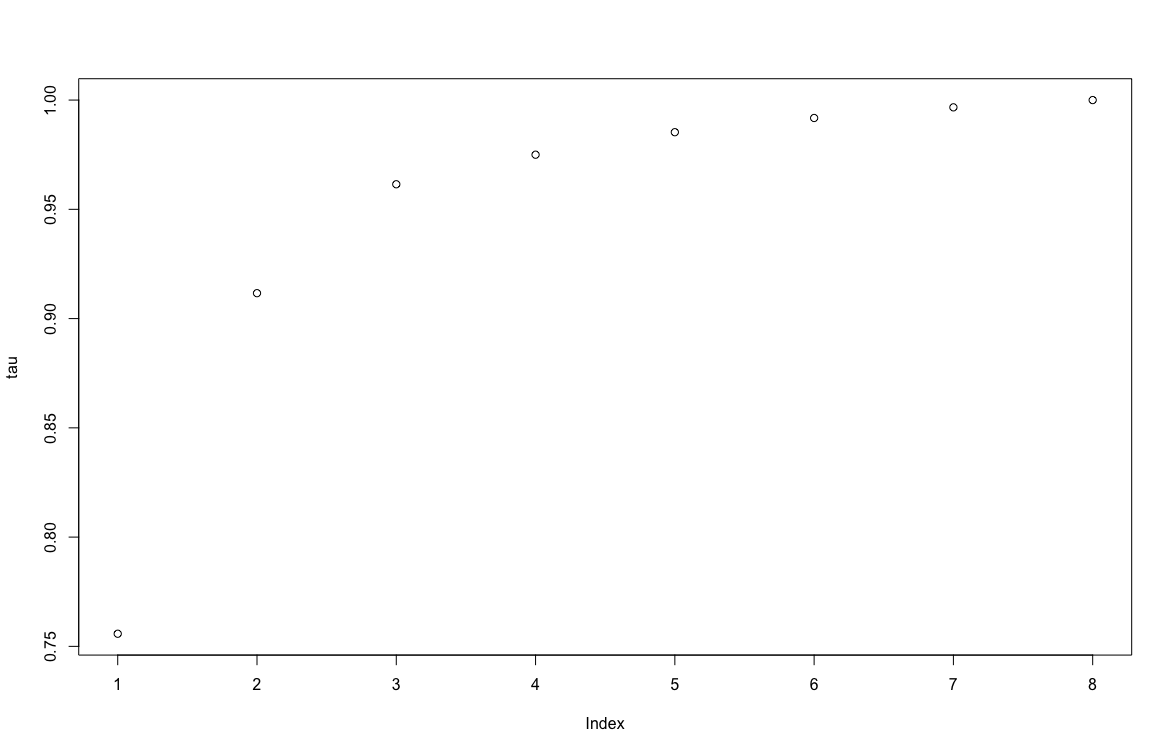
\includegraphics[scale=0.18]{2_1_var}
	\end{center}
	Wir sehen auch, dass die Variablen Design, Sporty, Value, Service und Safety mit $PC_1$ positiv korrelieren, während Price negativ mit $PC_1$ korreliert. Das ist auch klar, da ein billiges Auto keine teuren Features wie Service, Design, etc haben kann.
	\begin{center}
		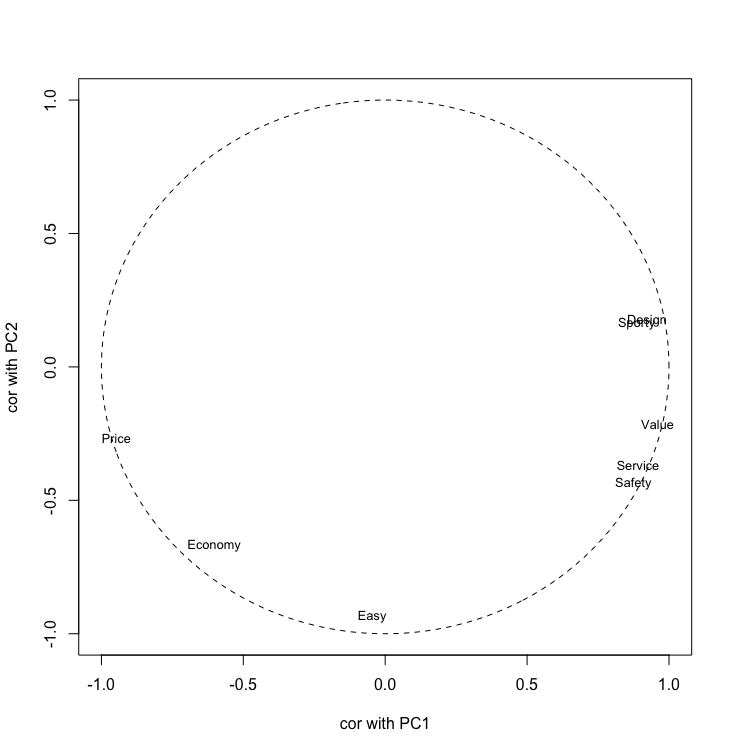
\includegraphics[scale=0.3]{2_1_cor}
	\end{center}
	Das wird auch noch mal im Biplot sichtbar, besonders teure Autos sind BMW, Ferrari und Jaguar, während Autos der Marken Wartburg und Trabi billig sind.
	\begin{center}
		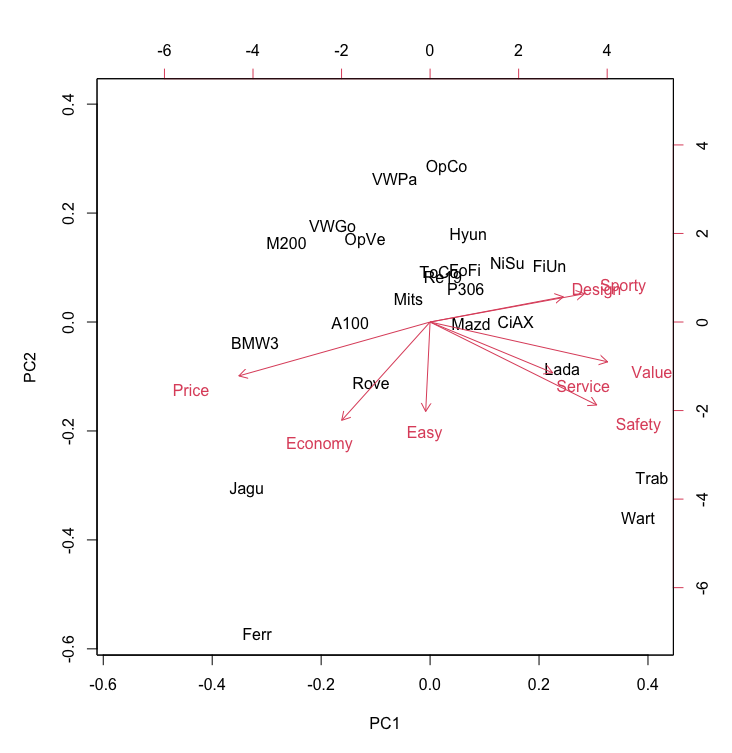
\includegraphics[scale=0.3]{2_1_biplot}
	\end{center}

	\section*{Task 2}
	\begin{lstlisting}
# normale lineare Regression
summary(lm(Price ~ 0 + ., data = carmean2))

# principle component regression
price = scale(carmean2[,4], center = TRUE, scale = FALSE)
PCs = prcomp(scale(carmean2[,-4], center = TRUE, scale = FALSE))$x[,1:2]
summary(lm(price ~ 0 + PCs))
	\end{lstlisting}
	Die normale lineare Regression liefert
	\begin{center}
\begin{tabular}{l c}
\hline
 & lineare Regression \\
\hline
Economy    & $0.61^{*}$ \\
           & $(0.28)$   \\
Service    & $0.34$     \\
           & $(0.47)$   \\
Value      & $-0.91$    \\
           & $(0.45)$   \\
Design     & $0.60$     \\
           & $(0.32)$   \\
Sporty     & $-0.05$    \\
           & $(0.34)$   \\
Safety     & $-0.42$    \\
           & $(0.32)$   \\
Easy       & $0.97$     \\
           & $(0.46)$   \\
\hline
R$^2$      & $0.98$     \\
Adj. R$^2$ & $0.98$     \\
Num. obs.  & $23$       \\
\hline
\multicolumn{2}{l}{\scriptsize{$^{***}p<0.001$; $^{**}p<0.01$; $^{*}p<0.05$}}
\end{tabular}
\end{center}
	Während die principle component regression folgende Werte liefert:
	\begin{center}
\begin{tabular}{l c}
\hline
 & principle component regression \\
\hline
PCsPC1     & $-0.52^{***}$ \\
           & $(0.03)$      \\
PCsPC2     & $-0.41^{***}$ \\
           & $(0.07)$      \\
\hline
R$^2$      & $0.93$        \\
Adj. R$^2$ & $0.93$        \\
Num. obs.  & $23$          \\
RMSE       & $0.31$        \\
\hline
\multicolumn{2}{l}{\scriptsize{$^{***}p<0.001$; $^{**}p<0.01$; $^{*}p<0.05$}}
\end{tabular}
\end{center}
	Man sieht, dass sich $R^2$ bzw. der adjustierte $R^2$ fast gleich sind, was wiederum bedeutet, dass man mit 2 PCs fast den ganzen Datensatz erklären kann.
	
	\section*{Task 3}
	\begin{lstlisting}
load("data/uscrime.rda")
pca2 = prcomp(uscrime[,3:9], center = TRUE, scale. = TRUE)
pca2
tau2 = cumsum(pca2$sdev^2)/sum(pca2$sdev^2)
plot(tau2)
biplot(pca2)
plot(cos((0:360)/180*pi), sin((0:360)/180*pi), type = "l", lty = "dashed", xlab = "cor with PC1", ylab = "cor with PC2")
text(cor(uscrime[,3:9], pca2$x)[,1:2], labels = colnames(uscrime[,3:9]), cex = 0.8)
plot(pca2$x[,1:2], col = c("orange", "green", "blue", "red")[uscrime$reg], xlab = "PC1", ylab = "PC2")
text(pca2$x[,1:2], labels = colnames(uscrime), col = c("orange", "green", "blue", "red")[uscrime$reg], cex = 0.8, pos = 4)
legend("topright", legend = levels(uscrime$reg) , col = c("orange", "green", "blue", "red"), pch = 20)
	\end{lstlisting}
	Liefert die folgenden Eigenwerte $\lambda_1 = 4.0767793$, $\lambda_2 = 1.4316417$, $\lambda_3 = 0.6311694$, $\lambda_4 = 0.3401460$, $\lambda_5 = 0.2483953$, $\lambda_6 = 0.1396704$, $\lambda_7 = 0.1321979$, dazu die folgenden PCs:
	\begin{align}
		\begin{array}{l}
			murder \\
			rape \\
			robbery \\
			assault \\
			burglary \\
			larceny \\
			autotheft
		\end{array}
		\left(\begin{array}{rrrrrrr}
			0.2761 & 0.6445 & -0.0095 & 0.3287 & -0.203 & -0.1002 & -0.5908 \\ 0.4214 & 0.1163 & -0.3601 & -0.2958 & 0.759 & 0.0652 & -0.1068 \\ 0.3875 & -0.046 & 0.6041 & -0.6451 & -0.1896 & -0.069 & -0.1608 \\ 0.3881 & 0.4562 & 0.0107 & 0.0669 & -0.1359 & -0.1004 & 0.7798 \\ 0.4364 & -0.2572 & -0.1554 & 0.1436 & -0.2916 & 0.7829 & -0.0269 \\ 0.3604 & -0.4009 & -0.5082 & -0.0481 & -0.3599 & -0.5609 & -0.0686 \\ 0.3539 & -0.3661 & 0.472 & 0.6007 & 0.3372 & -0.2079 & 0.012
		\end{array}\right) \notag
	\end{align}
	Auch hier nehmen wir wieder 2 PCs, diese erklären fast 80\% der Varianz:
	\begin{center}
		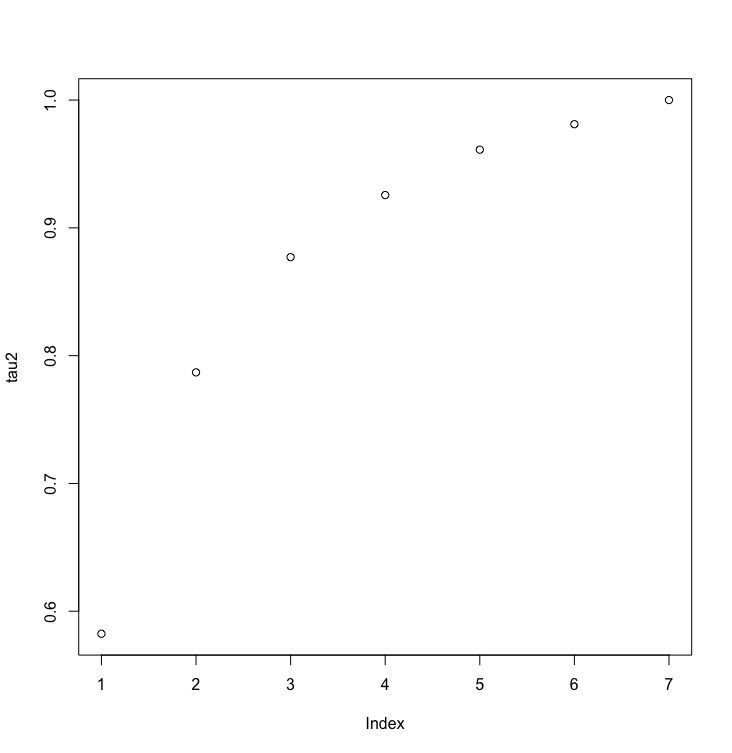
\includegraphics[scale=0.23]{2_3_var}
	\end{center}
	Im Korrelationsplot sehen wir, dass $PC_1$ angibt, ob eine Straftat vorliegt und $PC_2$ sagt uns, wie schwer diese ist:
	\begin{center}
		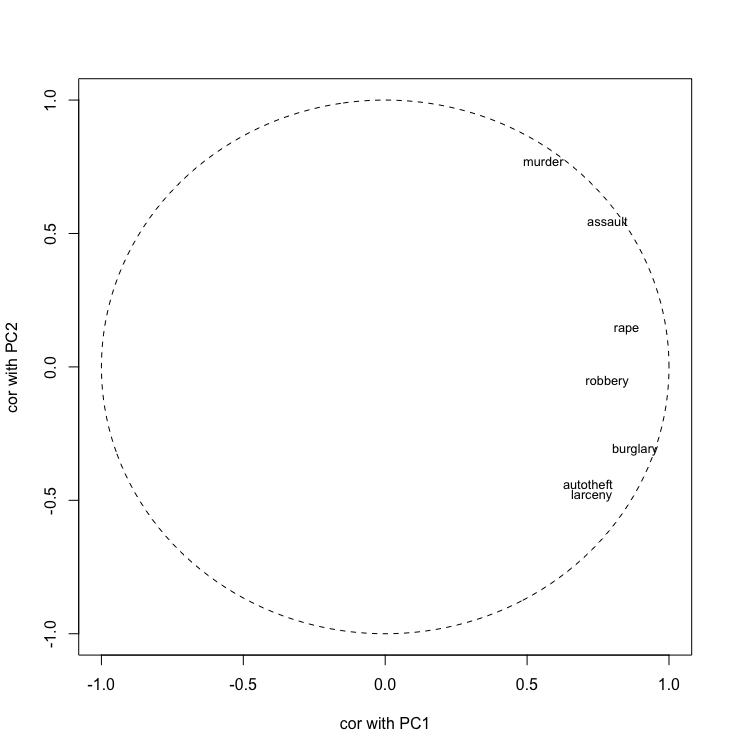
\includegraphics[scale=0.3]{2_3_cor}
	\end{center}
	Im Biplot sehen wir, dass es durchaus Unterschiede zwischen den Staaten gibt, in North Dakota gibt es am wenigsten Straftaten.
	\begin{center}
		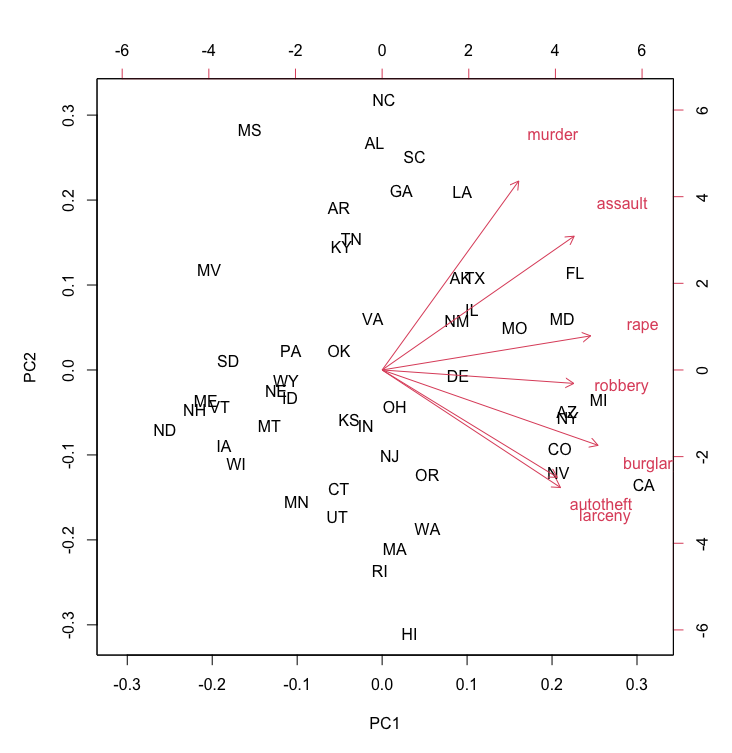
\includegraphics[scale=0.3]{2_3_biplot}
	\end{center}
	Man kann das ganze noch nach Region aufteilen, im Süden gibt es besonders schwere Straftaten:
	\begin{center}
		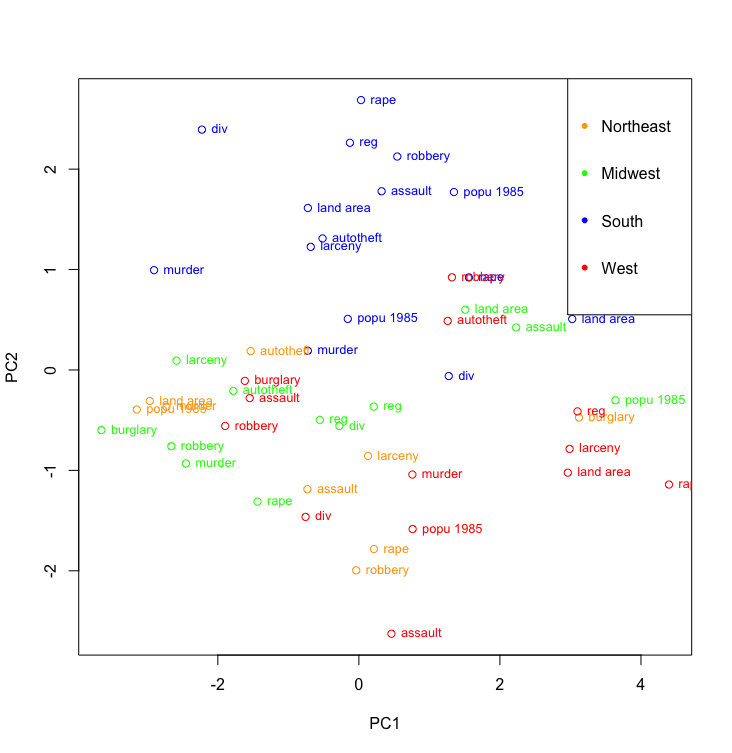
\includegraphics[scale=0.3]{2_3_location}
	\end{center}
\end{document}